\documentclass[aspectratio=169, plain, 14pt]{beamer}
\beamertemplatenavigationsymbolsempty
\setbeamertemplate{footline}[frame number]
\usepackage[utf8]{inputenc}
\usepackage[russian]{babel}
\usepackage[table]{xcolor}
\setbeamertemplate{itemize items}[circle]
\usepackage{ragged2e}
\usepackage{mathtools}
\usepackage{cleveref}
\usepackage{physics}

%My blocks
\setbeamercolor{block title}{fg=white,bg=blue!65!black}
\setbeamercolor{block body}{fg=black,bg=blue!10!white}
%%%%%%%%%%%%%%%%%%%%%%%%%%%%%%%%%%%

\title{Л4. Модель силовой установки}
\author{Сутурин Даниил}
\institute{ЦНИИХМ}
\date{\today}

\begin{document}
	
\begin{frame}
	\titlepage{}
\end{frame}
%%%%%%%%%%%%%%%%%%%%%%%%%%%%%%%%%%%%%%%%%
\begin{frame}{Силовая установка}
	\justifying\small
	В современной малой авиации все чаще появляются самолеты с электрической силовой установкой, что обусловлено развитием высокоемких аккумуляторных батарей
	\begin{columns}
		\column{0.5\linewidth}
		\begin{figure}
			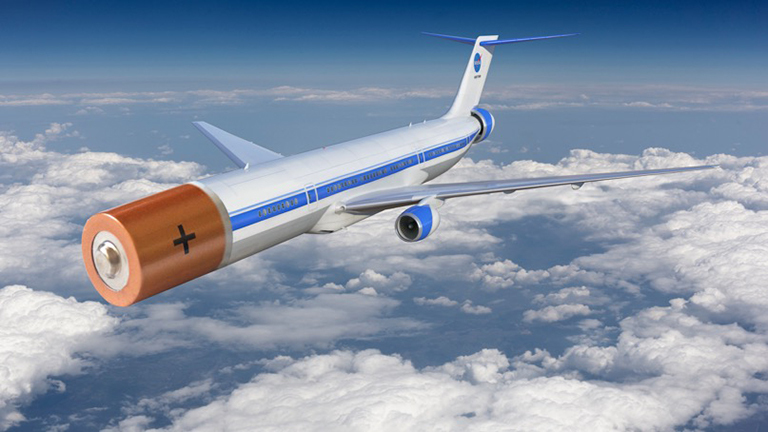
\includegraphics[width=0.9\textwidth]{FlyingBattery.jpg}
		\end{figure}
		
		\column{0.5\linewidth}
		\begin{figure}
			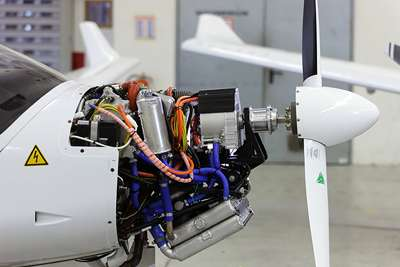
\includegraphics[width=0.9\textwidth]{ElectroMotor.jpg}
		\end{figure}
	\end{columns}

\end{frame}	
%%%%%%%%%%%%%%%%%%%%%%%%%%%%%%%%%%%%%%%%%%
\begin{frame}{Состав СУ}
	\justifying\small
	В нашей модели силовая установка элекрическая, состоящая из мотора и воздушного винта.
	\begin{columns}
		\column{0.5\linewidth}
		\begin{figure}
			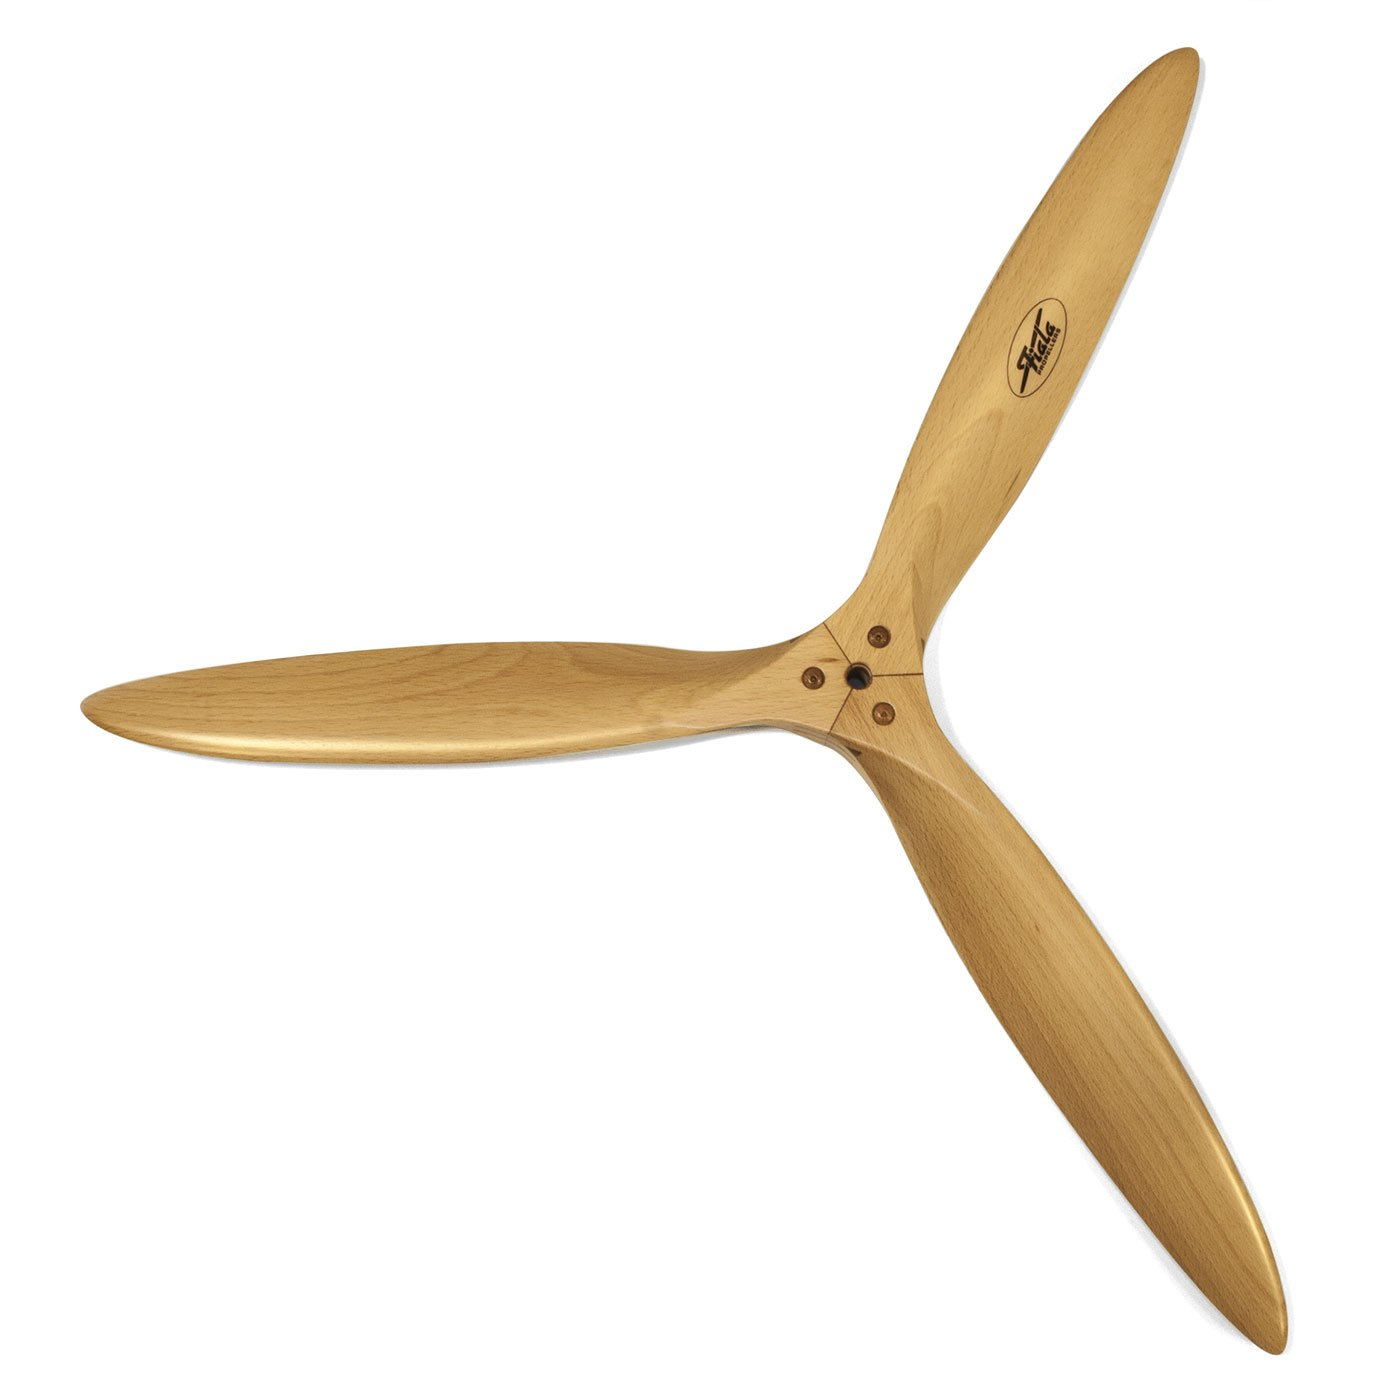
\includegraphics[width=0.8\textwidth]{prop.jpg}
		\end{figure}
		\column{0.5\linewidth}
		\begin{figure}
			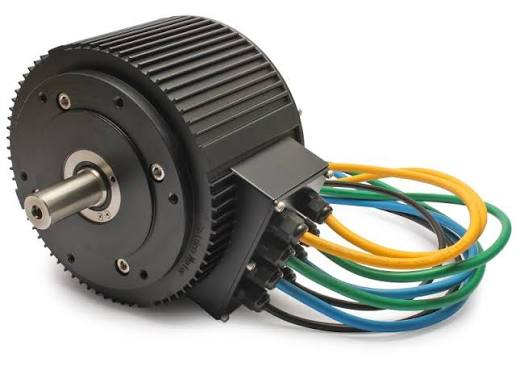
\includegraphics[width=0.8\textwidth]{BLDC.jpg}
		\end{figure}
	\end{columns}
\end{frame}
%%%%%%%%%%%%%%%%%%%%%%%%%%%%%%%%%%%%%%%%%%%%%%%
\begin{frame}{Модель мотора}
	\only<1>{
	\begin{columns}
		\justifying\small
		\column{0.4\textwidth}
		Рассмотрим модель бесколлекторного электромотора (BLDC). Состоит из токопроводящих обмоток (фаз) и постоянных магнитов, расположенных на роторе, а также датчиков Холла для контроля положения ротора.
		\column{0.6\textwidth}
		\begin{figure}
			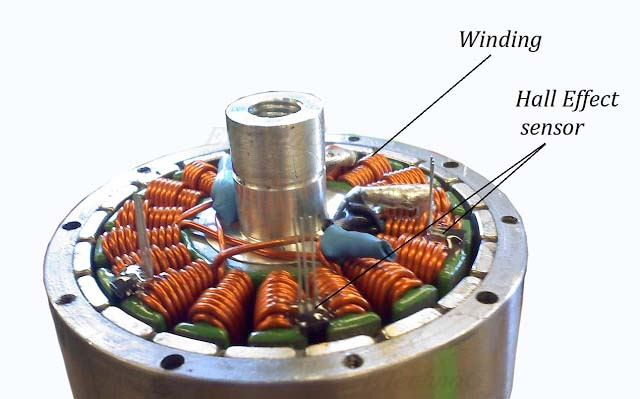
\includegraphics[width=1\linewidth]{InnerStructureBLDC.jpeg}
		\end{figure}
	\end{columns}
}
%%%%%%%%%%%%%%%%%%%%%%%%%%%%%%%%%%%%%%%%
\only<2>{
	\begin{columns}
		\column{0.5\linewidth}
		\begin{figure}
			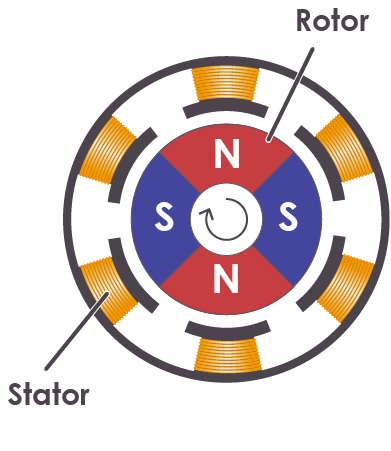
\includegraphics[width=0.9\linewidth]{Motor.png}
		\end{figure}
		\column{0.5\linewidth}
		\justifying\small
		На роторе находятся постоянные магниты с магниным моментом $\boldsymbol{p}_m$, который ориентирован вдоль оси вращения ротора. Обмотки при подаче на них тока создают магнитное поле эквивалентное соленоиду $\boldsymbol{B}_i$. При определенной схеме подачи тока (коммутации) на обмотки возникает момент $\boldsymbol{\tau}$, действующий на магнит:
		$$
		\boldsymbol{\tau} = \boldsymbol{p}_m \cross \sum{\boldsymbol{B}_i}, \\
		|\boldsymbol{B}_i| = \mu_0 n I,\\
		n - \text{плотность намотки витков}, \\
		I - \text{ток в обмотке}
		$$
	\end{columns}
}
%%%%%%%%%%%%%%%%%%%%%%%%%%%%%%%%%%%
\only<3>{
	\justifying\small
	При вращении ротора с магнитами и быстром переключении тока с одной фазы на другую происходит постоянное изменение магниного поля внутри мотора, что приводит к ЭДС индукции в обмотках мотора согласно закону Фарадея:
	$$
		E_{i} \propto -\frac{d\Phi}{dt} = -\frac{d\int{\boldsymbol{B}d\boldsymbol{S}} } { dt } \propto \Omega
	$$
	\justifying\small
	Чтобы учесть зависимость механического момента на роторе от тока и ЭДС индукции от угловой скорости вращения используют эквивалентную схему мотора и ряд параметров:
	\begin{columns}
		\column{0.4\linewidth}
		\begin{figure}
			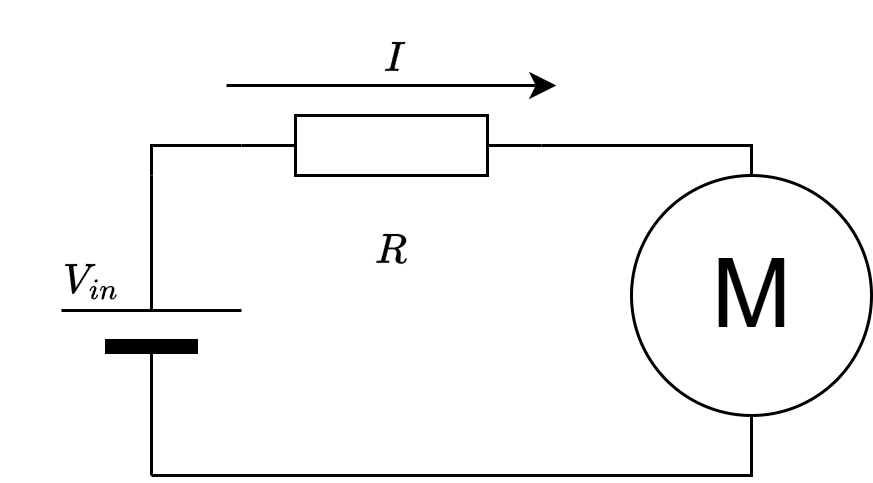
\includegraphics[width=0.75\linewidth]{MotorEquivalentScheme.png}
		\end{figure}
		\column{0.6\linewidth}
		$
		E_i = K_V\Omega, \quad K_V - \text{коэфф. ЭДС идукции [$\frac{B}{RPM}$]} \\
		Q_m = K_Q (I-i_0), \quad K_Q - \text{коэфф. момента [$\frac{H\cdot \text{м}}{A}$]} \\
		R - \text{сопротивление обмоток} \\
		V_{in} - \text{напряжение на обмотках} \\
		i_0 - \text{ток холостого хода}\\
		$
	\end{columns} 
}
%%%%%%%%%%%%%%%%%%%%%%%%%%%%%%%%%%%%
\only<4>{
	\justifying\small
	Применяя правило Кирхгофа для замкнутого контура эквивалентной схемы на слайде выше получаем основные соотношения для механического момента $Q_m$ на валу мотора, входного напряжения $V_{in}$ и КПД $\eta_m$:
	$$
	V_{in} - E_i = IR, \quad I = (V_{in} - K_V\Omega)/R
	$$
	\centering
	\boxed
	{
	Q_m = K_Q (I-i_0) = K_Q \left( \frac{(V_{in} - K_V\Omega)}{R} - i_0\right)   
	}
	\centering
	\boxed{
		\eta_m = \frac{\text{Механическая мощность}}{\text{Электрическая мощность}} = \frac{Q_m\Omega}{V_{in}I}
	}
}
\end{frame}
%%%%%%%%%%%%%%%%%%%%%%%%%%%%%%%%%%%%%%%%%%%%%%%%%%%%%%%
\begin{frame}{Модель воздушного винта}
\only<1>{
	\justifying\small
	Тяга $T_p$ и механический момент $Q_p$ винта:
	$$
	T_p(\Omega, C_T) = \frac{\rho D^4}{4\pi^2}\Omega^2 C_T
	$$
	$$
	Q_p(\Omega, C_Q) = \frac{\rho D^5}{4\pi^2}\Omega^2 C_Q,
	$$
	где безразмерные коэффициенты тяги $C_T$ и механического момента $C_Q$ учитывают зависимость от скорости набегающего потока на диск воздушного винта.
	\boxed{\text{статическая тяга $\neq$ тяга в полете}}
	$$
	J = \frac{2\pi V_a}{\Omega D} - \text{поступь винта}
	$$
	\centering
	\boxed{
	C_T = C_{T_0} + C_{T_1}J + C_{T_2}J^2, \quad C_Q = C_{Q_0} + C_{Q_1}J + C_{Q_2}J^2
	}
}
%%%%%%%%%%%%%%%%%%%%%%%%%%%%%%%%%%%%%%%%%%%%%%%%%
\only<2>{
\begin{figure}
	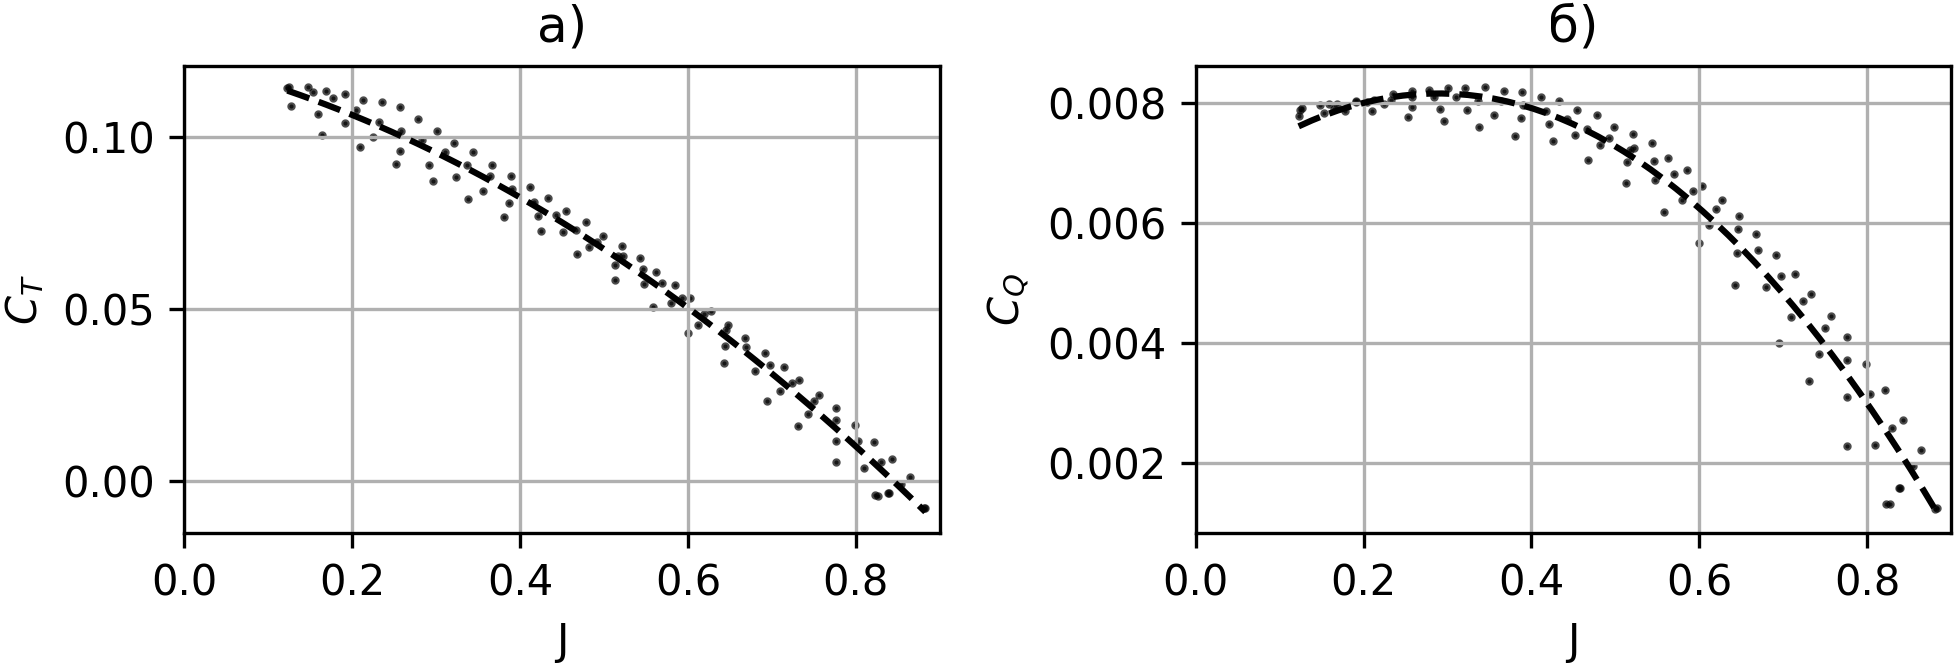
\includegraphics[width=1\textwidth]{TorqueThrustCoeff.png}
\end{figure}
}
%%%%%%%%%%%%%%%%%%%%%%%%%
\only<3>{
	\justifying\small
Воздушный винт жестко связан с валом мотора, поэтому $Q_p = Q_m$:
$$
\frac{\rho D^5}{4\pi^2}\Omega^2(C_{Q_0} + C_{Q_1}J + C_{Q_2}J^2) = K_Q \left( \frac{(V_{in} - K_V\Omega)}{R} - i_0\right)
$$
Решая квадратное уравнение относительно $\Omega$ при заданных $V_{in}$ и $V_a$:
$$
a\Omega^2 + b\Omega + c = 0, \quad \Omega = \frac{-b + \sqrt{b^2 - 4ac}}{2a}
$$
$$
a = \frac{\rho D^5}{4\pi^2}C_{Q_0}, \quad 
b = \frac{\rho D^4}{2\pi} C_{Q_1}V_a + \frac{K_V K_Q}{R}, \quad
c = \rho D^3 V_a^2 C_{Q_2} + K_Q i_0 - \frac{K_Q}{R}V_{in} 
$$
определим тягу и механический момент винта
}
%%%%%%%%%%%%%%%%%%%%%%%%%%%%%%%%%%%%%%%%%%%%%%
\only<4>{
\begin{columns}
	\column{0.5\textwidth}
	\begin{figure}
		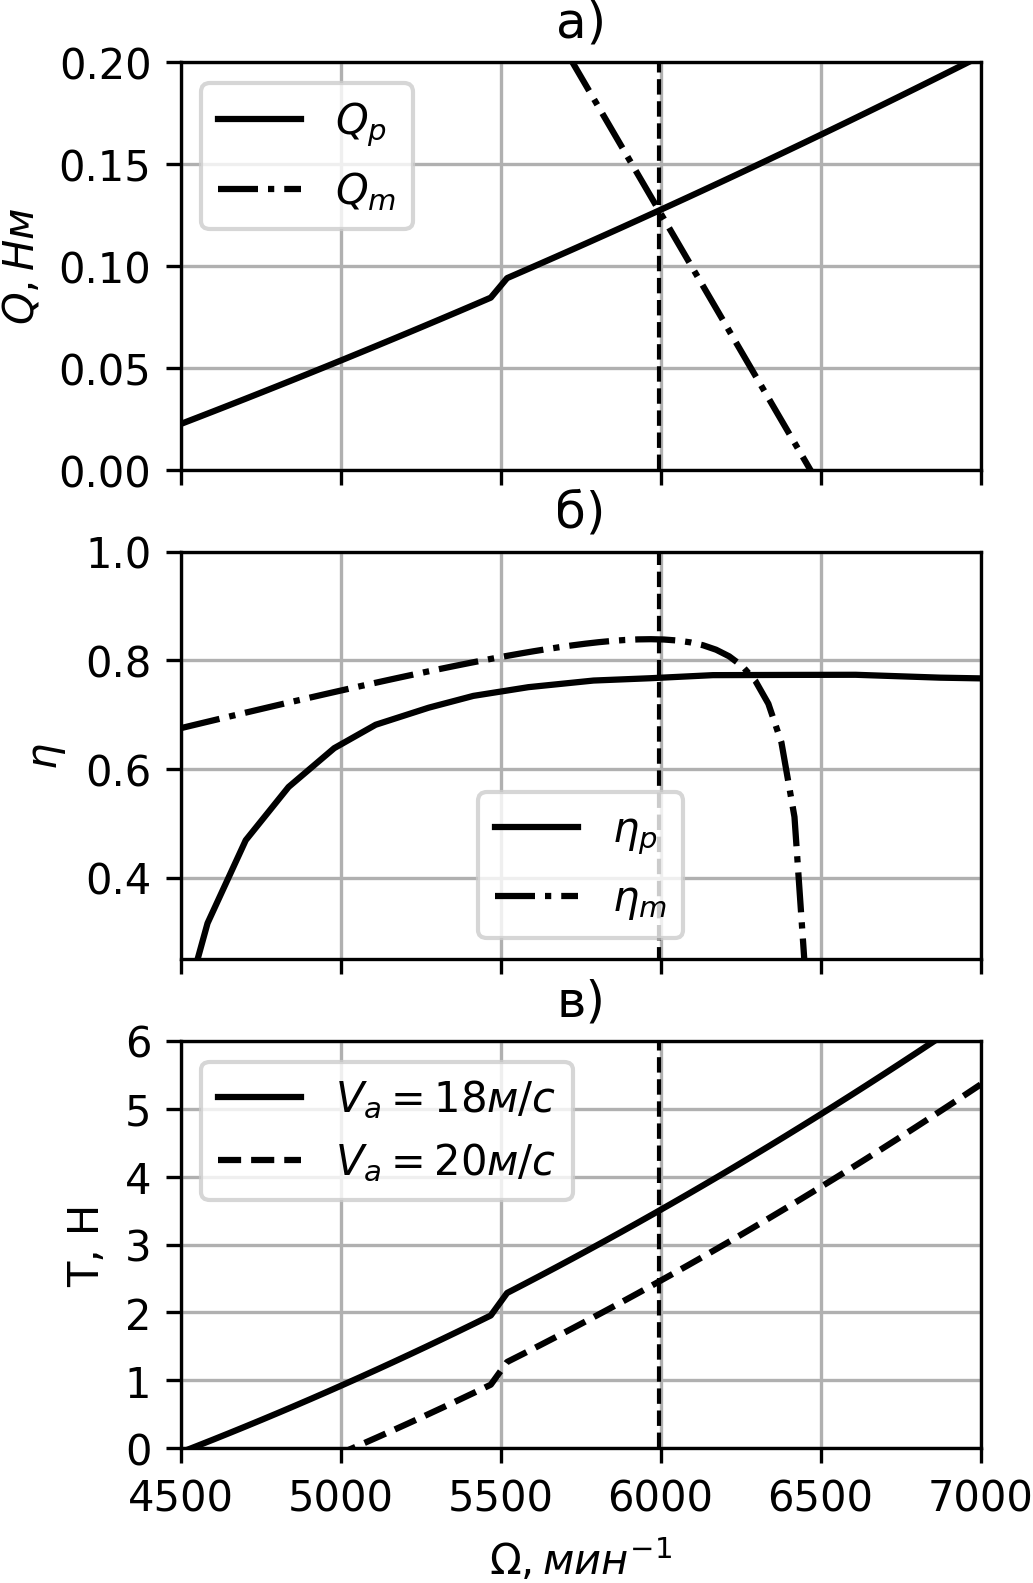
\includegraphics[width=0.7\linewidth]{MotorMatching.png}
	\end{figure}
	\column{0.5\textwidth}
	\begin{figure}
		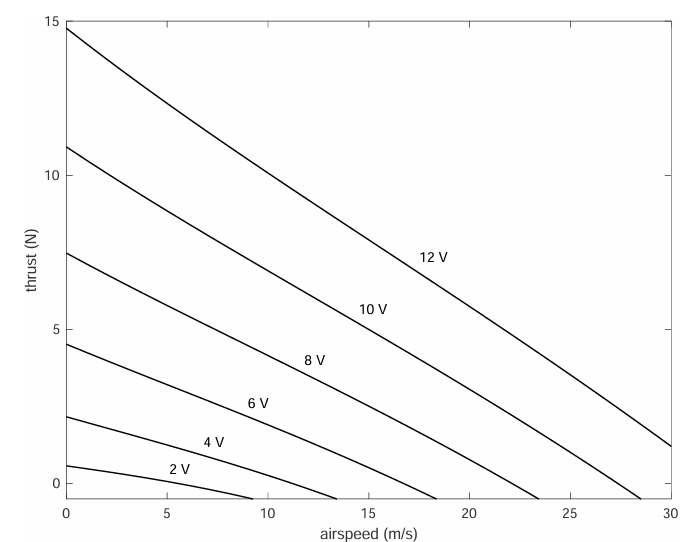
\includegraphics[width=0.65\linewidth]{ThrustVSSpeed.png}
		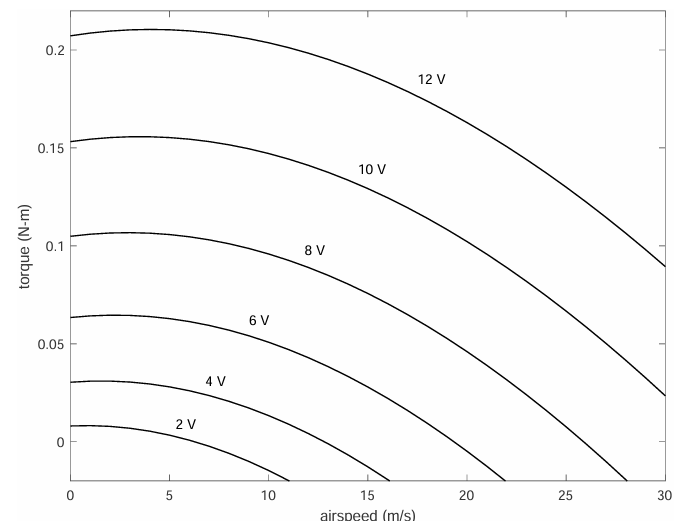
\includegraphics[width=0.65\linewidth]{TorqueVSSpeed.png}
	\end{figure}
	
	
\end{columns}
}
\end{frame}
%%%%%%%%%%%%%%%%%%%%%%%%%%%%%%%%%%%%%%
\begin{frame}{Тяга и момент винта}
	\justifying\small
	Сила тяги и механический момент винта в ССК имеют вид:
	$$
	\boldsymbol{f}^b_{propulsion} = \begin{pmatrix}
		T_p \\ 0 \\ 0
	\end{pmatrix}, \quad \boldsymbol{M}^b_{propulsion} = \begin{pmatrix}
		-Q_p \\ 0 \\ 0
	\end{pmatrix}
	$$
\end{frame}
\end{document}